\subsection{Czemu interesują nas takie konstrukcje?}
\epigraph{A~komu to potrzebne? A~dlaczego?}{\textit{Pani z~Internetu, zapytana, czy należy w~Polsce zalegizować marihunaen}}
Mogłoby się wydawać, że liczba chromatyczna jest w jakiś sposób własnością lokalną grafu. To znaczy, oczywiście widzimy, że jeśli graf ma liczbę klikową $\omega$, to musimy użyć przynajmniej $\omega$ kolorów do jego pokolorowania. No dobra, ale może gdybyśmy lokalnie pokolorowali podgrafy będące dużymi klikami, to pozostałe części grafu już damy radę załatwić jakąś rozsądną liczbą dodatkowych kolorów? Prawda? Nieprawda. Okazuje się, że istnieją grafy, które nie zawierają nawet trójkątów, czyli mają $\omega < 3$, ale mają też dowolnie dużą liczbę chromatyczną. Czyli niestety życie (przynajmniej jeśli dla kogoś życie opiera się na optymalnym kolorowaniu grafów) nie jest takie proste\dots
\subsection{Co będziemy konstruować?}
Pokażemy trzy sposoby zrobienia ciągu grafów $G_3, G_4, \ldots$ (zaczynamy od $3$~bo dla $0$, $1$ i~$2$ nie dzieje się nic ciekawego) takiego, że dla dowolnego $n \geq 3$ będą zachodzić dwie własności:
\begin{itemize}
	\item $\omega\pars{G_n} = 2$
	\item $\chi\pars{G_n} \geq n$
\end{itemize}
Warto zwrócić uwagę, że $n$~\emph{nie będzie} liczbą wierzchołków w~takim grafie. Pamiętajmy --- ten ciąg grafów indeksujemy \emph{liczbą chromatyczną}, która nas interesuje, nie liczbą wierzchołków. Liczba wierzchołków wyjdzie w~praniu i~będzie zupełnie inna.

W każdym z~trzech sposobów zaczniemy od położenia $G_3 = C_5$. Wszystko się zgadza --- $C_5$ nie zawiera trójkąta i~ma $\chi = 3$, bo jest cyklem nieparzystej długości. Resztę ciągu skonstruujemy rekurencyjnie.
\subsection{Konstrukcja Mycielskiego}
Załóżmy sobie, że mamy już $G_n$, które spełnia wszystkie własności, jakie chcieliśmy. Chcemy teraz zrobić $G_{n + 1}$. W~tym celu najpierw weźmiemy wierzchołki z~$G_n$ --- nazwijmy je $v_1, v_2, \ldots, v_N$, gdzie $N = \left|V\pars{G_n}\right|$ (pamiętajmy tylko, że $N \neq n$). Doróbmy sobie jeszcze ,,kopie'' tych wierzchołków, tzn. odpowiadające im nowe wierzchołki, które nazwiemy $v_1', v_2', v_N'$, i~dorzućmy jeszcze specjalny wierzchołek $v^\ast$. Czyli, podsumowując, kładziemy
\begin{equation*}
	V\pars{G_{n + 1}} \coloneqq \left\{v_1, v_2, \ldots, v_N\right\} \cup \left\{v_1', v_2', \ldots, v_N'\right\} \cup \left\{v^\ast\right\}
\end{equation*}
A~jak będzie z~krawędziami? Po pierwsze, krawędzie między oryginalnymi wierzchołkami grafu $G_n$ zostają jak były. Po drugie, każdy wierzchołek będący kopią łączymy z~wierzchołkiem specjalnym. Po trzecie, \emph{nie łączymy} żadnych dwóch kopii. I~po czwarte, każdą kopię łączymy z~sąsiadami odpowiadającego jej oryginału (czyli zapewniamy, że kopia ma takie samo sąsiedztwo jak oryginał, poszerzone jedynie o $v^\ast$). Formalnie:
\begin{equation*}
	E\pars{G_{n + 1}} \coloneqq E\pars{G_n} \cup \left\{v_iv^\ast : i \in [N]\right\} \cup \left\{v_i'v_j : i, j \in [N] \land v_iv_j \in E\pars{G_n} \right\}
\end{equation*}
Wyglądać to będzie mniej więcej tak:

\begin{figure}[H]
	\centering
	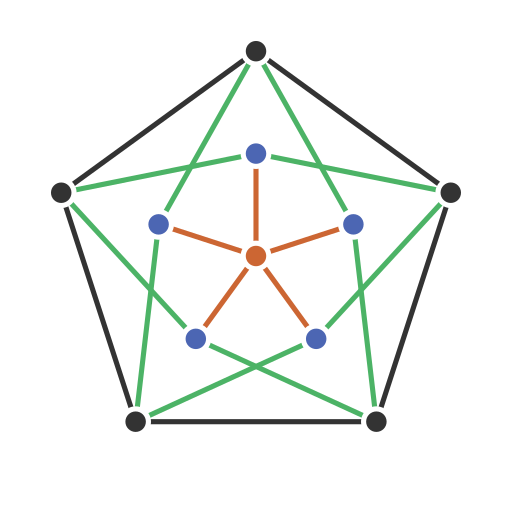
\includegraphics[scale=0.5]{images/mycielski_graph.png}
	\caption{Graf $G_4$ w konstrukcji Mycielskiego}
\end{figure}

Przekonajmy się teraz, że stworzony $G_{n + 1}$ posiada dwie cechy, których oczekiwaliśmy:
\begin{itemize}
	\item $\omega\pars{G_{n + 1}} = 2$, czyli nie ma trójkątów. Zastanówmy się:
	      \begin{itemize}
		      \item na pewno $v^\ast$ nie jest w~żadnym trójkącie, bo jego sąsiadami są tylko kopie, a~żadne dwie kopie nie są połączone
		      \item z~tego samego powodu żaden potencjalny trójkąt nie zawiera dwóch wierzchołków będących kopiami
		      \item trójkąt nie może składać się z~samych oryginałów, bo założyliśmy, że w~oryginalnym $G_n$ nie było trójkątów
	      \end{itemize}
	      Zatem gdyby istniał trójkąt, to byłby on w~postaci $v_iv_j'v_k$, dla pewnych $i, j, k \in [N]$. Wtedy mielibyśmy oczywiście $v_iv_k \in E\pars{G_{n + 1}}$, $v_j'v_i \in E\pars{G_{n + 1}}$ oraz $v_j'v_k \in E\pars{G_{n + 1}}$.\\
	      Ale pamiętajmy, że graf $G_{n + 1}$ skonstruowaliśmy tak, żeby oryginalny wierzchołek i~jego kopia miały to samo sąsiedztwo (nie licząc $v^\ast$). Zatem skoro $v_j'v_i \in E\pars{G_{n + 1}}$ oraz $v_j'v_k \in E\pars{G_{n + 1}}$, to zachodzi $v_jv_i \in E\pars{G_n}$ oraz $v_jv_k \in E\pars{G_n}$. Krawędzi między oryginałami nie ruszaliśmy, więc skoro $v_iv_k \in E\pars{G_{n + 1}}$ to również $v_iv_k \in E\pars{G_n}$.\\
	      Ale z~tego wszystkiego wychodzi, że w~oryginalnym $G_n$ istniał już trójkąt $v_iv_jv_k$, a~przecież założyliśmy, że tak nie jest. Uzyskana sprzeczność dowodzi, że w~$G_{n + 1}$ nie ma trójkątów.
	      \qed
	\item $\chi\pars{G_{n + 1}} \geq n + 1$.
	      Załóżmy, że tak nie jest, tzn. $\chi\pars{G_{n + 1}} \leq n$. Weźmy zatem kolorowanie $c$, które o~tym świadczy i~poprawnie koloruje $G_{n + 1}$ używając nie więcej niż $n$~kolorów. Przyjrzyjmy się teraz wierzchołkom-kopiom: widzimy na nich maksymalnie $n - 1$ kolorów. Dlaczego? Gdyby zużywały one $n$ kolorów, to zabrakłoby wolnego koloru na $v^\ast$, który przecież jest połączony ze wszystkimi kopiami.\\
	      Świetnie, to teraz stwórzmy sobie kolorowanie $c'$ grafu $G_n$, które dla każdego $i \in [N]$ będzie działać bardzo prosto:
	      \begin{equation*}
		      c'\pars{v_i} = \begin{cases}
			      c\pars{v_i}  & \iff c\pars{v_i} \neq c\pars{v^\ast} \\
			      c\pars{v_i'} & \iff c\pars{v_i} = c\pars{v^\ast}
		      \end{cases}
	      \end{equation*}
	      Innymi słowy: jeśli dany wierzchołek miał w~kolorowaniu $c$~taki kolor, jak specjalny wierzchołek $v^\ast$, to dajemy mu kolor jego kopii, a~w~przeciwnym przypadku zostawiamy taki kolor, jaki był. Zauważmy, że $c'$ jest poprawnym kolorowaniem $G_n$. Dlaczego? Gdyby nie było, to znaczyłoby, że istnieje krawędź $v_iv_j$ taka, że $c'\pars{v_i} = c'\pars{v_j}$. Są trzy potencjalne wyjaśnienia tej sytuacji:
	      \begin{itemize}
		      \item w~kolorowaniu $c$~wierzchołki $v_i$ i~$v_j$ już miały ten sam kolor i~pozostał on niezmieniony --- ale to jest niemożliwe, bo kolorowanie $c$~było poprawne
		      \item w~kolorowaniu $c$~wierzchołki $v_i$ i~$v_j$ miały ten sam kolor $c\pars{v^\ast}$, i~dla obydwu uległ on zmianie na ten sam kolor --- niemożliwe, jak wyżej
		      \item w~kolorowaniu $c$~wierzchołki wierzchołki miały różne kolory, przy czym dokładnie jeden z~nich miał kolor $c\pars{v^\ast}$. Przyjmijmy bez straty ogólności, że był to $v_i$. Skoro zatem $c'\pars{v_i} = c'\pars{v_j}$, a~$c\pars{v_i} = c\pars{v^\ast}$, to mamy $c\pars{v_i'} = c'\pars{v_j} = c\pars{v_j}$. Ale to jest niemożliwe, bo skoro jest krawędź $v_iv_j$, to jest też krawędź $v_i'v_j$, a~w~poprawnym kolorowaniu $c$~nie mogło być dwóch sąsiednich wierzchołków w~tym samym kolorze.
	      \end{itemize}
	      Uzyskane sprzeczności dowodzą, że $c'$~rzeczywiście jest poprawnym kolorowaniem $G_n$ przerobionym z~kolorowania $c$, które używało nie więcej, niż $n$~kolorów. Ale zauważmy, że w~$c'$~pozbyliśmy się  jednego z~kolorów, mianowicie $c\pars{v^\ast}$. Zatem $c'$~jest poprawnym $\pars{n - 1}$-kolorowaniem grafu $G_n$, co jednak jest niemożliwe, bo przecież założyliśmy, że $\chi\pars{G_n} \geq n$. Uzyskana sprzeczność dowodzi ostatecznie, że istotnie $\chi\pars{G_{n + 1}} \geq n + 1$.
	      \qed
\end{itemize}
\subsection{Konstrukcja Tutte'a}
Ponownie zakładamy, że mamy działające $G_n$ i~chcemy zrobić $G_{n + 1}$. Przyjmijmy $N = \left|V\pars{G_n}\right|$. Ta konstrukcja jest bardzo prosta: najpierw tworzymy sobie $n \cdot \pars{N - 1} + 1$ zupełnie nowych wierzchołków --- nazwijmy je \emph{wierzchołkami głównymi}. Teraz przy każdym $N$-elementowym podzbiorze tych wierzchołków tworzymy kopię $G_n$ i~łączymy wierzchołki główne z~odpowiadającymi im wierzchołkami z~kopii $G_n$ (w~dowolnym porządku, byle każdy wierzchołek główny z~podzbioru miał dokładnie jednego kolegę w~odpowiadającej temu podzbiorowi kopii). Najłatwiej to zobaczyć na poniższym rysunku:

\begin{figure}[H]
	\centering
	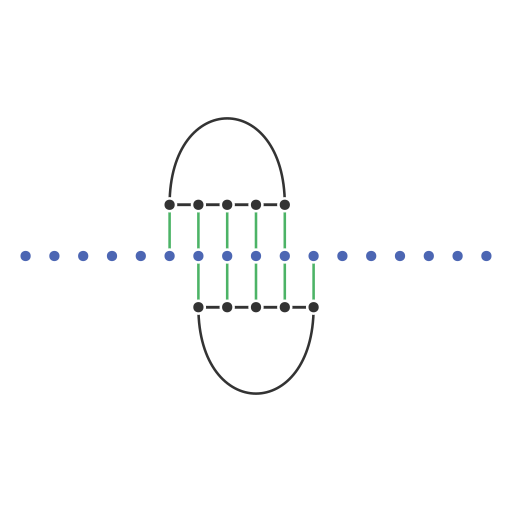
\includegraphics[scale=0.5]{images/tutte_graph.png}
	\caption{Fragment $G_4$ w konstrukcji Tutte'a}
\end{figure}

Między poszczególnymi kopiami $G_n$ nie dajemy żadnych krawędzi. Podobnie nie dajemy żadnych krawędzi między wierzchołkami głównymi. I~gotowe --- mamy nasze $G_{n + 1}$! Przyjrzyjmy się, czemu taki graf spełnia nasze wymagania:
\begin{itemize}
	\item brak trójkątów --- oczywiście żadnego trójkąta nie ma:
	      \begin{itemize}
		      \item w~żadnej kopii $G_n$, bo założyliśmy, że $G_n$ jest bez trójkątów
		      \item pomiędzy kopiami $G_n$, bo powiedzieliśmy, że różnych kopii w~żaden sposób nie łączymy
		      \item wśród wierzchołków głównych, bo między nimi nie ma krawędzi
	      \end{itemize}
	      Zatem jedyny możliwy trójkąt musiałby mieć jeden wierzchołek główny i~dwa wierzchołki z~kopii. Ale te dwa z~kopii nie mogą być w~jednej kopii $G_n$, bo każdy wierzchołek główny ma dokładnie jednego kolegę w~każdej kopii. Nie mogą też być w~różnych kopiach $G_n$, bo aby domknąć trójkąt, musiałyby się łączyć, a~między kopiami nie ma krawędzi. Zatem w~$G_{n + 1}$ nie istnieją trójkąty.
	      \qed
	\item $\chi\pars{G_{n + 1}} \geq n + 1$. Załóżmy, że tak nie jest, czyli $\chi\pars{G_{n + 1}} \leq n$. Weźmy zatem kolorowanie, które o~tym świadczy. Ponieważ jest $n \cdot \pars{N - 1} + 1$ głównych wierzchołków, to z~zasady szufladkowej musi istnieć tam $N$~wierzchołków, które mają taki sam kolor, powiedzmy $k$. Rozważmy teraz kopię skonstruowaną przy tym $N$-elementowym podzbiorze wierzchołków głównych. Żaden z~wierzchołków w~tej kopii nie może mieć koloru $k$, ponieważ jest połączony z~odpowiadającym mu wierzchołkiem głównym. A~to oznacza, że ta kopia $G_n$ została pokolorowana nie więcej niż $n - 1$ kolorami. Ale to jest przecież niemożliwe, bo założyliśmy, że $\chi\pars{G_n} \geq n$. Uzyskana sprzeczność pokazuje, że istotnie $\chi\pars{G_{n + 1}} \geq n + 1$.
	      \qed
\end{itemize}

\subsection{Konstrukcja Zykova}
Również zakładamy, że mamy działające $G_n$. Będziemy tworzyć $G_{n + 1}$. Na dobry początek zróbmy sobie $n$~rozłącznych kopii grafu $G_n$. Teraz dla każdego możliwego wyboru, wyróżniającego po jednym wierzchołku z~każdej kopii, dodajemy jeden wierzchołek ,,na dole'' i~łączymy go z~tymi wyróżnionymi. Żadnych innych krawędzi nie dodajemy. Ponownie, najlepiej to zobaczyć na rysunku:

\begin{figure}[H]
	\centering
	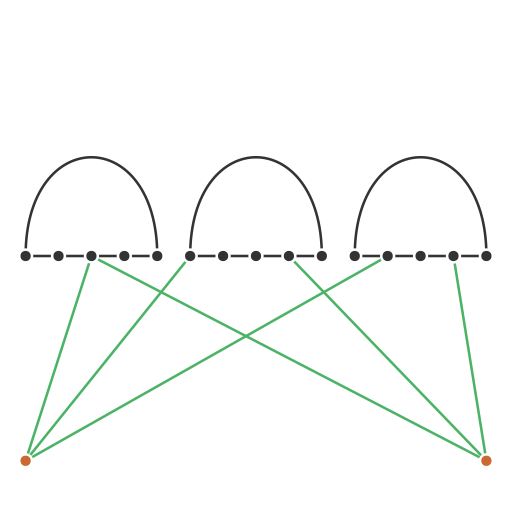
\includegraphics[scale=0.5]{images/zykov_graph.png}
	\caption{Fragment $G_4$ w konstrukcji Zykova}
\end{figure}

To będzie nasze $G_{n + 1}$. Zbadajmy, czemu to działa:
\begin{itemize}
	\item brak trójkątów --- na pewno trójkąt nie znajdzie się:
	      \begin{itemize}
		      \item w~żadnej kopii $G_n$, bo z~założenia nie ma tam trójkątów
		      \item pomiędzy różnymi kopiami $G_n$, bo nie są one wcale połączone
		      \item wśród wierzchołków ,,na dole'', bo nie ma między nimi żadnych krawędzi
	      \end{itemize}
	      Zatem jedyny potencjalny trójkąt musiałby mieć jeden wierzchołek na dole i~dwa w~kopiach $G_n$. Te dwa ,,górne'' nie mogą być jednak w~tej samej kopii $G_n$, bo każdy wierzchołek z~dołu w~danej kopii ma \emph{dokładnie jednego} sąsiada. Nie mogą też być w~różnych kopiach $G_n$, bo musiałyby być połączone, a~przecież kopie się nie łączą. Czyli żaden trójkąt nie może się pojawić w~$G_{n + 1}$.
	      \qed
	\item $\chi\pars{G_{n + 1}} \geq n + 1$. Pokażemy, że nie da się pokolorować $G_{n + 1}$ używając $n$-kolorów. Załóżmy do dowodu nie wprost, że jest to możliwe, i~weźmy takie poprawne $n$-kolorowanie. Powiedzmy, że te kolory to $1, 2, \ldots, n$. Oczywiście każda kopia $G_n$ używa wszystkich $n$~kolorów, bo $\chi\pars{G_n} \geq n$. Zatem z~pierwszej kopii wybierzmy dowolny wierzchołek w~kolorze $1$, z~drugiej kopii dowolny wierzchołek w~kolorze $2$, \dots, z~$n$-tej kopii wierzchołek w~kolorze $n$. To jest wybór po jednym wierzchołku z~każdej kopii, więc na dole jest wierzchołek połączony z~nimi wszystkimi. Ups\dots Ale to oznacza, że zabraknie na niego wolnego koloru, bo dla każdego z~dostępnych $n$~kolorów ten ,,dolny'' wierzchołek jest połączony z~wierzchołkiem w~tym kolorze ,,na górze''. Uzyskana sprzeczność dowodzi nierówności $\chi\pars{G_{n + 1}} \geq n + 1$.
	      \qed
\end{itemize}